\chapter{Results}
\label{results}
This section will detail the major simulations that were made, and the conclusions we can draw from them in
regards to their impact on the overall transmission of the system. To begin, we started with the simplest
model: just a straight waveguide according to the specs outlined in \cref{setup}. We simulated waveguides of
two different lengths, one that is on the order of the characteristic input wavelength and one that is much
larger. As it turns out, the scale of the waveguide makes a significant impact when it comes to the
transmission parameter we measure. 

With the straight waveguide simulated, we then proceed to add one bend to the structure, and investigate its
effects on the overall transmission of the waveguide. In particular, we first start by introducing a
sharp bend, then we introduced a rounded bend and compared the results of the transmission against each
other.

\section{Straight Waveguide}

\begin{figure}
	\centering
	\begin{subfigure}{0.4\textwidth}
		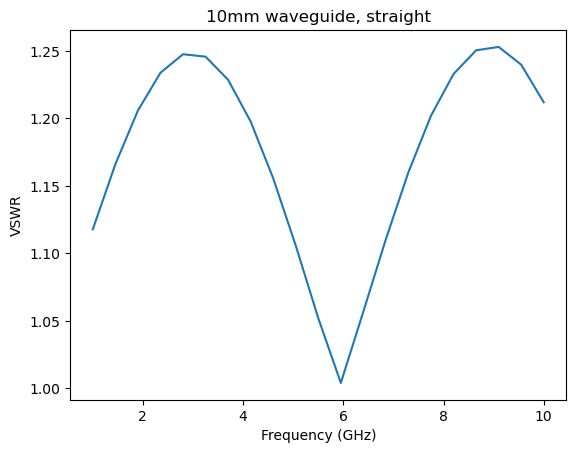
\includegraphics[scale=0.5]{images/plots/short-finiteconductivity.png}
		\caption{}
		\label{short-finiteconductivity}
	\end{subfigure}
	\hspace{2cm}
	\begin{subfigure}{0.4\textwidth}
		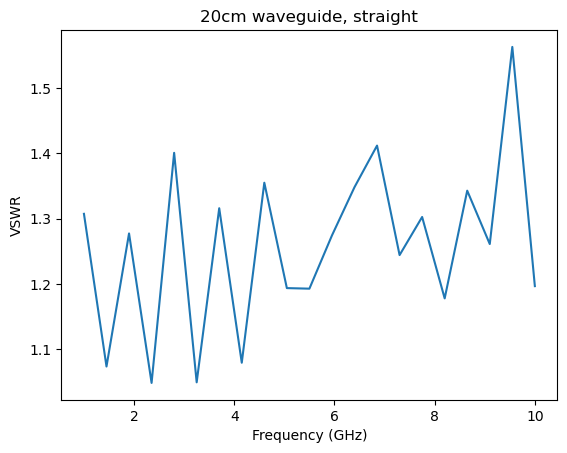
\includegraphics[scale=0.5]{images/plots/long-finiteconductivity.png}
		\caption{}
		\label{long-finiteconductivity}
	\end{subfigure}
	\caption{Plots of the VSWR for the (a) short and (b) long waveguides. Notice that in the short case,
	there is one resonant frequency around 6 GHz, and in the case of the long waveguide there are many more
	resonant frequencies.}
	\label{straight-waveguides}
\end{figure}
 
To begin, we look at the straight waveguide. Here, we simulated two waveguides of two different lengths, one
of length 10mm, and the other 20cm. We picked these particular lengths because we wanted to investigate how
the transmission of the waveguide changes when the length of the waveguide is on the order of, and also much
larger than the wavelength of the incoming wave. 

A plot of the VSWR for the short and long simulation are shown in \cref{straight-waveguides}. As shown in
\cref{short-finiteconductivity}, the VSWR plot shows one particular frequency at which the VSWR is minimized,
at around 6 GHz. This makes sense given the geometry of the CPW, since using the typical formula \( \lambda
= c / f \) means that a 6 GHZ signal corresponds to a wavelength of 40mm. Given that our straight waveguide
is a multiple of the wavelength, it means that this particular wave propagates at a "resonant" frequency,
hence the low reflection coefficient. By comparison, none of the other frequencies are resonant, meaning they
will all reflect a wave of some amplitude, explaining their higher VSWR values. This fact is also further
shown when we slightly vary the length of the waveguide, as shown in \cref{longbox-waveguides}. In this case,
we've increased the length of the short waveguide to 13mm from 10, and as a result in its VSWR plot we now
see two minima, indicating that there are two resonant frequencies, at roughly 4.5 and 9 GHz.

\begin{figure}
	\centering
	\begin{subfigure}{0.4\textwidth}
		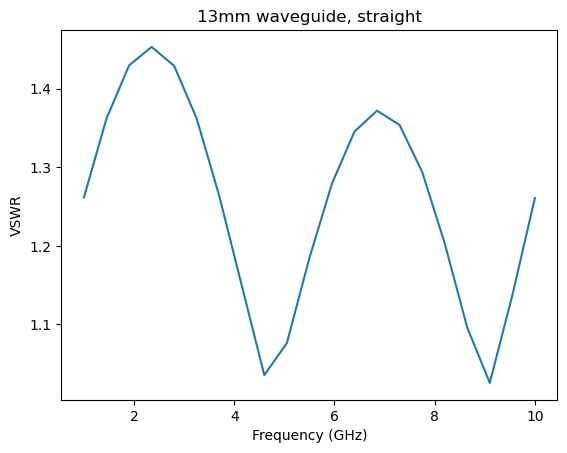
\includegraphics[scale=0.5]{images/plots/short-finitecond-longbox.png}
		\caption{}
		\label{short-finitecond-longbox}
	\end{subfigure}
	\hspace{2cm}
	\begin{subfigure}{0.4\textwidth}
		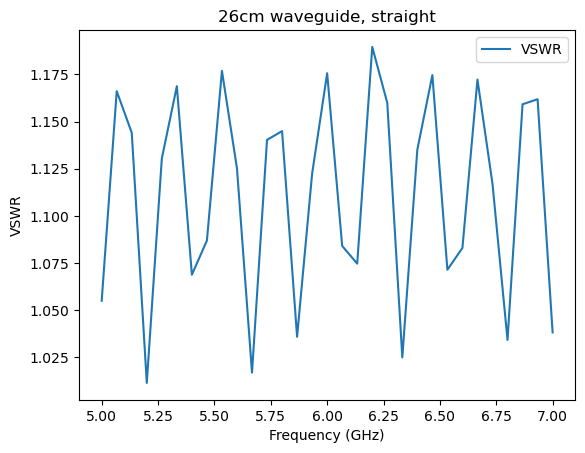
\includegraphics[scale=0.5]{images/plots/long-finitecond-longbox.png}
		\caption{}
		\label{long-finitecond-longbox}
	\end{subfigure}
	\caption{Plots of the VSWR for the (a) short and (b) long waveguides, which are slightly longer than
		those used in \cref{short-finiteconductivity} and \cref{long-finiteconductivity}. Notice the
		difference in the number of minima in each case, strongly suggesting that there is a resonance effect in
	the waveguide.}
	\label{longbox-waveguides}
\end{figure}

The same resonance logic can be applied to the longer waveguide: we just have more resonance frequencies because the
waveguide is longer, but the principle still applies. However, there are some interesting features in the
long waveguide that we cannot yet explain: firstly, the region between 5 and 7 GHz seems to have no resonance
frequencies, and the oscillatory nature of the VSWR begins to break down at higher frequencies. Interestingly
enough, this phenomenon is present in \cref{long-finiteconductivity}, but not present in
\cref{long-finitecond-longbox}, possibly suggesting that this is simply a numerical artifact and not a
physical phenomenon. The latter observation of degrading VSWR with increasing frequency is a common phenomenon 
seen in many of our simulations, but we do not have a concrete answer for why this occurs. 

Another observation we made was that due to the fact that our surrounding box is conducting, the incoming
wave seemed to also exhibit standing wave modes with the surrounding box, which we call "box modes". These
box modes are particularly problematic, because the reflection of the wave off the surrounding box can
interact again with the wave traveling through the waveguide, causing interference in the signal. Evidence of
these box modes are shown in \cref{boxmode}, where we can clearly see the nonzero electric field that
oscillates between the central CPW and the surrounding box on the sides. The mitigation of these box modes
are an entirely different area of investigation, which we will not dive into here. This could explain the
anomalies we find in the VSWR plot for the long waveguide, but we are unsure at the moment. 

\begin{figure}
	\centering
	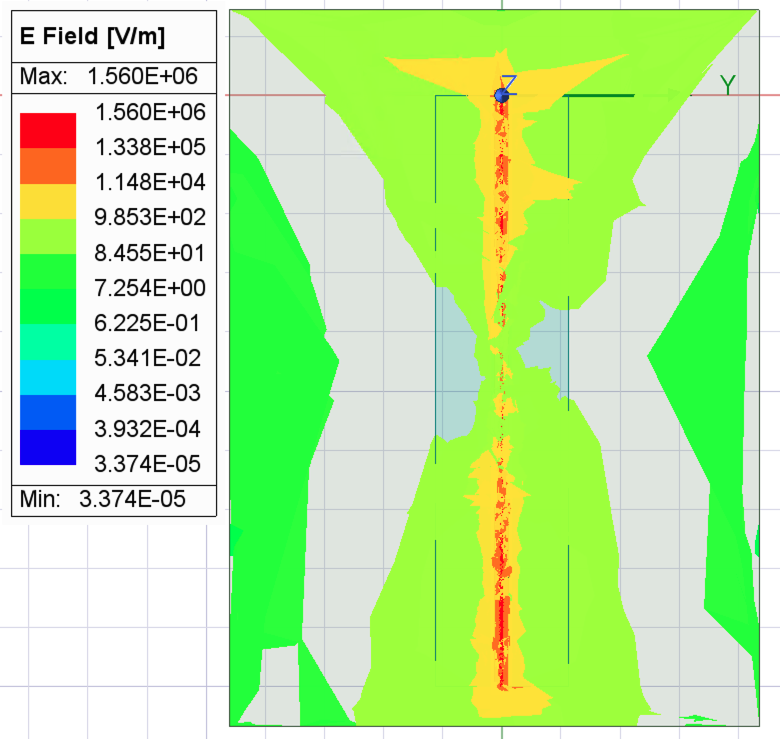
\includegraphics[scale=0.3]{images/model/short-boxmode.png}
	\caption{Plot showing the electric field solution for a wave of a particular frequency through the short
	waveguide. Of note is the oscillatory nature of the electric field in the horizontal direction, showing
	interaction between the CPW and the surrounding box and indicating the presence of box modes.}
	\label{boxmode}
\end{figure}

Finally, I want to end this section by discussing the importance of simulating these simple waveguides.
Although they are non-representative of the waveguides we use in the actual detectors, these simulations help
us grasp a basic understanding of how the transmission in a waveguide behaves numerically. This is especially
true in our case where many mathematical approximations need to be made to arrive at an analytic solution, so
numerical solutions may produce different results than our theoretical results. Furthermore, these
simulations also help us establish a baseline for the expected behavior when we add complications to the
waveguide, as we will see in the following section. 
 

\section{Adding Bends}
Here, we will add one complexity to our simulation by introducing a bend into the waveguide. The reason we
chose to focus on this particular feature compared to others is because when ultimately designing a KID
detector, we would ideally want to fit as many KIDs onto our substrate as possible, and the most
straightforward way to do
that is to have a "meandering" feedline that snakes across the material, like in \cref{feedline}. As a
result, it is important to investigate the effect of bends on our CPW. In particular, we investigate two
kinds of bends: first, we introduce a sharp \( 90^{\circ} \) bend, and also a rounded bend. Further, as the
ultimate goal of this project is to investigate the viability of the slow-wave structure from
\cite{hosaengkimWireBondFreeTechnique2009}, it is therefore important to first understand the effects of a
bend first. 

\subsection{Sharp Bends}
\cref{sharp-bends}

\begin{figure}
	\centering
	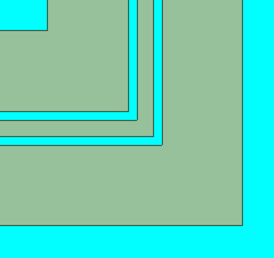
\includegraphics[scale=0.5]{images/model/sharp-bend.png}
	\caption{Sharp bend introduced to the waveguide.} 
	\label{sharp-bend}
\end{figure}

The simplest kind of bend we can introduce is a \( 90^{\circ} \) bend, shown in \cref{sharp-bend}. In order
to make the model as close to the straight waveguide as possible, we introduce the bend exactly halfway
through the waveguide, and ensure that the \textit{total} length of the waveguide remains the same compared
to the straight waveguide. For example, in the case of the 10mm waveguide, this means that the wave travels
5mm, takes the bend, and travels the remaining 5mm. 

The simulated results are shown in \cref{sharp-bends}. Of note in these simulations is the fact that in the
case of the short waveguide, the presence of the bend doesn't really seem to affect the VSWR plot very much,
at least in terms of the resonance. However, the standing wave ratio for the non-resonant frequencies is much
worse than \cref{short-finiteconductivity}, reaching a maximum VSWR of roughly 1.40 compared to 1.25. One
possible explanation for this is that in the case of the bent waveguide, the coupling effect to the
surrounding box is stronger (as there is less distance for the wave to travel from one port to the other,
geometrically speaking), and therefore this could result in more interference especially in the non-resonant
frequencies. 

The same conclusion cannot be said for \cref{long-finitecond-bend-sharp}, where we see a significant difference
between it and \cref{long-finiteconductivity}. In particular, the resonances seem to not exist for low
frequencies, and seems to be more frequent for higher frequencies. The latter observation could be explained
by the fact that because the distance to the bend is half that of the full waveguide, this leads to twice the
number of resonances. The former observation, however, we do not currently have an explanation for.   

\begin{figure}
	\centering
	\begin{subfigure}{0.4\textwidth}
		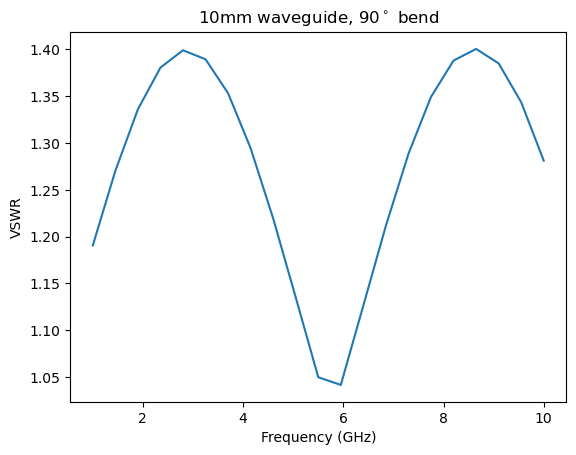
\includegraphics[scale=0.5]{images/plots/short-finitecond-bend-sharp.png}
		\caption{}
		\label{short-finitecond-bend-sharp}
	\end{subfigure}
	\hspace{2cm}
	\begin{subfigure}{0.4\textwidth}
		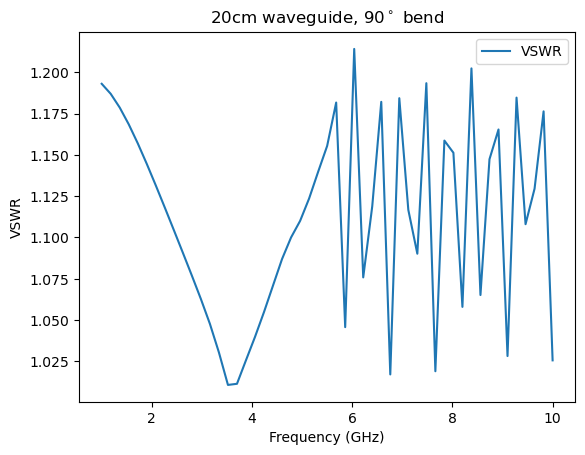
\includegraphics[scale=0.5]{images/plots/long-finitecond-bend-sharp.png}
		\caption{}
		\label{long-finitecond-bend-sharp}
	\end{subfigure}
	\caption{Plots of the VSWR for the (a) short and (b) long waveguides with a \( 90^{\circ} \) bend
		included. Notice that in the case of the short waveguide, the VSWR plot looks nearly identical to
	that of the straight waveguide, whereas that of the long waveguide does not.}
	\label{sharp-bends}
\end{figure}

Despite these differences however, the magnitude of the VSWR for the long waveguide does not seem to be
affected by the bend very much. Our primary hypothesis for this phenomenon goes back to \cref{conformal-map}.
In particular, using the same process outlined in \cref{conformal-map}, we can create a conformal map for the
dielectric constant of the bent waveguide and "straighten" it out, which leads to the mapping shown in
\cref{conformal-color}. As shown in the figure, we can see that introducing a bend into our waveguide is
equivalent to altering the dielectric constant in the waveguide -- this argument can also be made
intuitively, if you imagine "bending" the waveguide and making it straight, then the outer corner would be compressed
while the inner corner will be stretched which leads to a variation in the dielectric constant. 

Now, in principle, this should change the impedance of the waveguide. However, because the wavelengths that
we deal with are far larger than the size of this feature, we believe that the wave simply "skips" over such
a feature, which is why we don't see a significant change in the VSWR plot when we introduce the bends.  

\begin{figure}
	\centering
	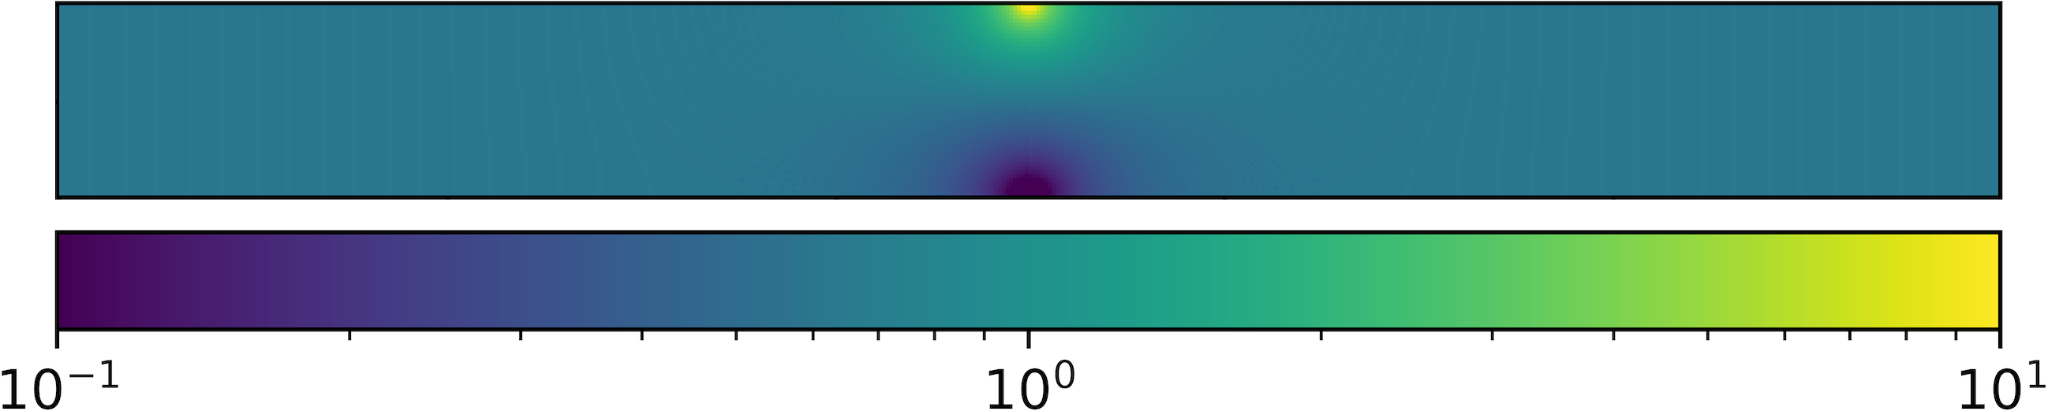
\includegraphics[width = 0.7\textwidth]{images/model/straight-color.png}
	\caption{Dielectric constant of the bent waveguide after a conformal mapping. Notice that the
		introduction of a bend manifests as a variation in the dielectric constant of the waveguide, which
	alters its impedance.} 
	\label{conformal-color}
\end{figure}

\subsection{Rounded Bends}
\label{rounded-bend}

\begin{figure}
	\centering
	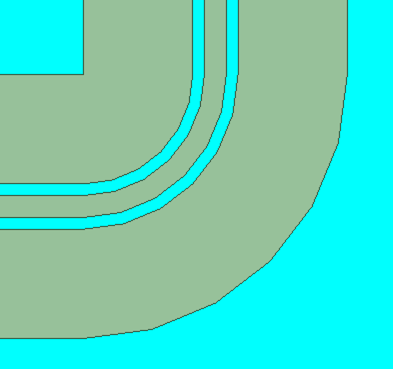
\includegraphics[scale=0.4]{images/model/small-round-bend.png}
	\caption{Rounded bend introduced to the waveguide.}
	\label{round-bend-small}
\end{figure}

Now, we move on to the third simulation: changing the type of bend from a sharp \(
90^{\circ} \) bend to a rounded one. The motivation for this is twofold: firstly, in the case of a sharp
bend, the location of the bend has a different impedance than the rest of the waveguide, because the gap
ratio slightly distorts due to the geometry of the bend. This phenomenon is eliminated with a rounded
waveguide, as we are able to maintain the size of the gap between the center and ground at all points. In
theory, we initially believed that this would result in better transmission. 

The bend structure we used is shown in \cref{round-bend-small}. We designed the bend so that the gap between
the center and ground lines are maintained, which in theory means that the impedance should not change over
the course of this bend. The corresponding VSWR plots are shown in \cref{round-bend-plot}, and we can
identify some significant differences between this and those shown in \cref{sharp-bends}. Firstly, in the
short waveguide, the VSWR for non-resonant frequencies is much larger than that in the case of a sharp bend,
indicating that the rounded bend contributes to more reflection than the sharp bend. This is rather
surprising, considering that we believed the rounded bend to be unilaterally better than the sharp bend.
We do have a hypothesis for this, which we will elaborate on later.   

\begin{figure}
	\centering
	\begin{subfigure}{0.4\textwidth}
		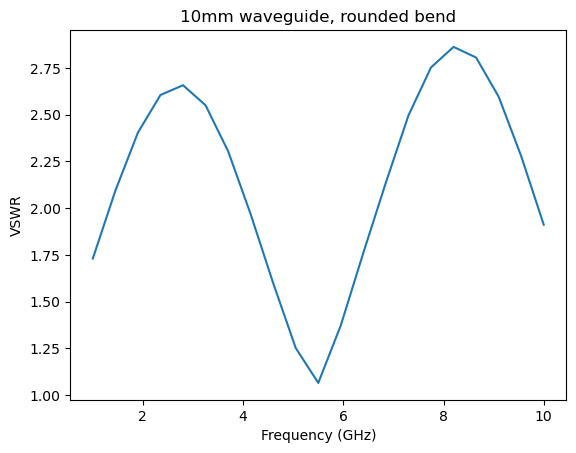
\includegraphics[scale=0.5]{images/plots/short-finitecond-bend-round.png}
		\caption{}
		\label{short-finitecond-bend-round}
	\end{subfigure}
	\hspace{2cm}
	\begin{subfigure}{0.4\textwidth}
		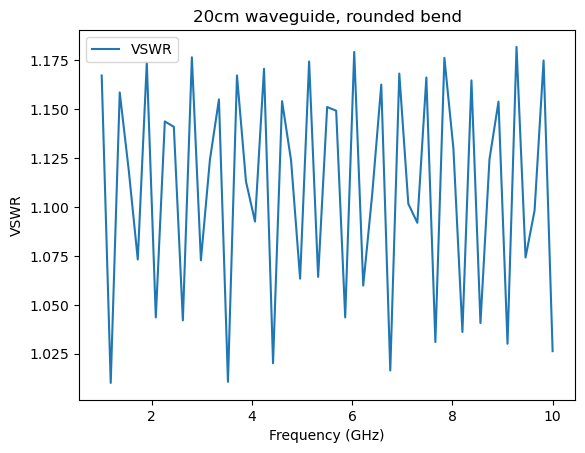
\includegraphics[scale=0.5]{images/plots/long-finitecond-bend-round.png}
		\caption{}
		\label{long-finitecond-bend-round}
	\end{subfigure}
	\caption{VSWR plots for the (a) short waveguide and (b) long waveguide, with a rounded bend. Notice that
	in the case of the short waveguide, the resonant frequency is untouched, but the VSWR for non-resonant
frequencies is much worse.}
	\label{round-bend-plot}
\end{figure}

The rounded bend has also affected the long waveguide in interesting ways -- firstly, the resonances at low
frequencies are present, unlike the plot shown in \cref{long-finitecond-bend-sharp}. However, this seems to
be about the only difference that is noticeable by eye. In terms of magnitude, the VSWR seems to match pretty
well with that of the \cref{long-finitecond-bend-sharp}, which seems to indicate that in this case, the
difference between a sharp and round bend does not really affect the overall transmission. We suspect this
could be due to the size of the feature: on a large scale, small differences like rounding out the bend should not do
much to the overall transmission because the feature size is small, hence why we don't see much variation in
the long waveguide but we do see changes in the short waveguide. 

\subsection{Large Round Bends}

The fourth and final simulation we conducted was a variation on the rounded bend. To fully investigate the
effect of the rounded bend, we decided to increase the radius of the bend. Theoretically, this has the
effect of "smoothening" out the bend even further compared to the earlier iterations, as the bend rounds a
larger corner and thus bends slower. Again, we preserve quantities like the gap between the center and
ground, so that the impedance of the CPW remains constant throughout.   

\begin{figure}
	\centering
	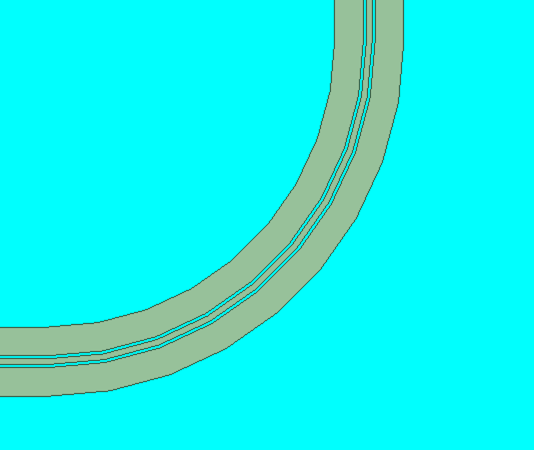
\includegraphics[scale=0.3]{images/model/large-bend.png}
	\caption{Example of the large rounded bend we introduced.}  
	\label{large-bend}
\end{figure}

A figure showing the modification to the bend is shown in \cref{large-bend}. Notice that here, the turning
radius of the bend is much larger than that in the previous section, and as a result the waveguide bends much
more smoothly. Our motivation behind studying this bend was to investigate the effect of "smoothening out"
the bending process, to see if this made the transmission of the waveguide better, as this would mitigate
some of the reflection that was present in the previous waveguides. 

\begin{figure}
	\centering
	\begin{subfigure}{0.4\textwidth}
		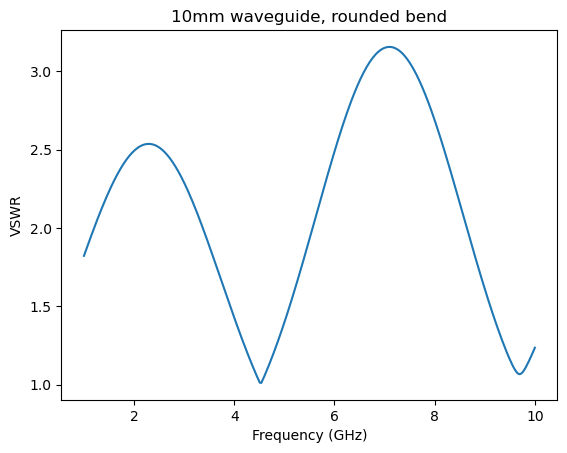
\includegraphics[scale=0.5]{images/plots/short-finitecond-round-big.png}
		\caption{}
		\label{short-finitecond-bend-round-big}
	\end{subfigure}
	\hspace{2cm}
	\begin{subfigure}{0.4\textwidth}
		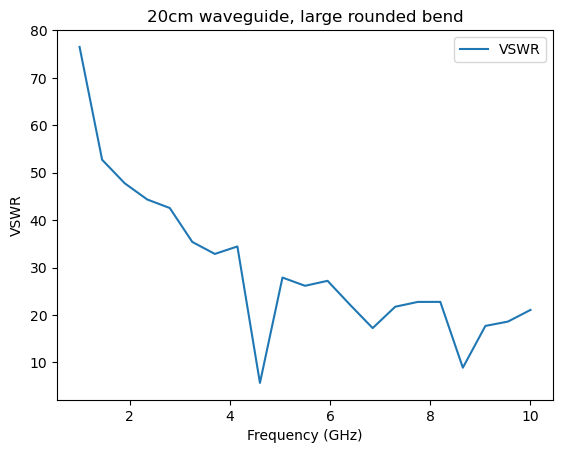
\includegraphics[scale=0.5]{images/plots/long-finitecond-round-big.png}
		\caption{}
		\label{long-finitecond-bend-round-big}
	\end{subfigure}
	\caption{VSWR plots for the (a) short waveguide and (b) long waveguide, with a larger rounded bend.
	Notice that here, we have drastic changes in both VSWR plots, compared to the previous plots in
\cref{sharp-bends} and \cref{round-bend-plot}.}
	\label{round-bend-big}
\end{figure}

The VSWR plots for these two simulations are shown in \cref{round-bend-big}. Interestingly, these plots look
significantly different, and in the case of the long waveguide, significantly worse in terms of transmission
compared to the simulations with the smaller bends. Our leading hypothesis in why this occurs goes back to
our discussion on conformal mappings in \cref{sharp-bends}. In particular, at the end of that section we
detailed how we believe that as long as the distortion to the dielectric constant is much smaller than the
wavelength of the signal, then the overall transmission is unlikely to be affected by the variations as the
wave would "skip over" these differences. For that same reason, when we introduce a large bend whose size is
no longer negligible, it appears that this has a drastic effect on the transmission of the waveguide. 

This leads us to the primary result that we've been able to conclude thus far: in terms of creating a
waveguide that minimizes the interference observed by impedance perturbation, it is more effective to choose
a bend that is small rather than one that better maintains the ratio \( a / b \) and yet has an extent comparable
to the wavelength. At first, this conclusion may seem
counter-intuitive since we are inclined to believe that gradually changing the bend should allow the wave to
bend nicely through the waveguide and minimize reflection, we find that this hypothesis is clearly false, as
our simulations and \cref{round-bend-big} clearly shows.
 
  
 

 
  
